\chapter{Overview of Simultaneous Localization and Mapping}
\label{cha:Overview}

\section{Overview of SLAM}
\label{sec:SLAM_parts}
Simultaneous Localization and Mapping, commonly abbreviated as SLAM, is concerned with the problem of a mobile robot building a map of the unknown environment, while at the same time navigating the environment using the map. A common way to formulate the SLAM problem is that a robot executes controls and accumulates observations of its environment taking into consideration that all measurements are corrupted by noise. The readings can be modeled as probability distribution functions. Both the pose of the robot and the location of the environmental features can also be considered to have probability distributions. Initially the variance of the robot pose is small because the initial pose is generally assured to be known to some level of accuracy. However as the robot moves around the environment, the pose estimate deteriorates due to accumulation of errors. The position of objects in the environment are assumed to have a large variance the first time they are seen, but with subsequent re-observation, the assurance of their position increases reducing the variance of their probability distribution. This approach to SLAM is called probabilistic SLAM. 

\begin{figure}
\centering
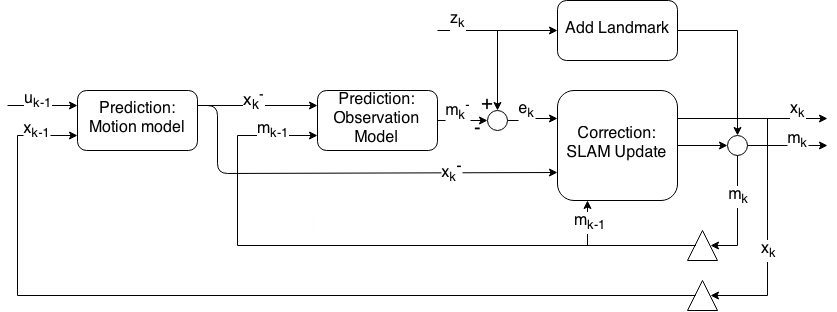
\includegraphics[width=\textwidth]{SLAM_diagram}
\caption{Block diagram of probabilistic SLAM process.}
\label{fig:SLAM_diagram}
\end{figure}

Most probabilistic SLAM methods follow the same structure. At every discrete time step $ k $, the inputs to the SLAM algorithm are: i) the control input to the robot $ u_{k-1} $ and ii) the environmental features detected by the sensors $ z_k $. The desired outputs of the SLAM algorithm are: the estimated robot pose $ x_k $, and the positions of landmarks or a map, represented by $ m_k $ . The general structure every probabilistic SLAM algorithm follows, is represented by the block diagram in Figure \ref{fig:SLAM_diagram}. First, the current pose estimate is calculated according to the motion model of the robot. This model uses the previous pose estimate and the last control input to compute the new estimated pose represented by $ x_k^- $. Then, the current measurement is estimated by an observation model. This observation model uses the current pose estimate and the previous landmark positions to make a prediction of the current measurement represented by $ m_k^- $. To obtain the error signal, the estimated measurement is subtracted from the real measurement $ z_k $. This error signal, represented by $ e_k $, together with the pose estimate and the previous landmark positions is used in the SLAM update step. The update step is used to improve the pose estimate and to update the landmark positions. This is usually done by some filter, such as Rao-Blackwellized Particle Filter (RBPF), an Extended Kalman Filter (EKF), or similar. After this step, new landmarks can be added to the map. 

\subsection{Pose Prediction}

The first step of SLAM is the prediction of the robot's state. The prediction is based upon known information about the robot's own motion model. This information about the robot's movement can be gathered using sensors such as encoders or by using the control signals sent to the robot's localization system or a combination of both. We assume that the position of the robot using GPS or someother global/local sensor is not available. These sensors which estimate the movement of the robot are termed \textit{proprioceptive} sensors. The movement information, even if attained from the sensors, is referred to as the \textit{control} inputs.

During the prediction step, the uncertainty of the robot's position is also updated. The maximum error can be approximated based on the movement of the robot and a predetermined error model. The error accumulates, resulting in increase of the uncertainty in the robot's position. The error and motion models change based on the expected environment and the robot's specific platform and hardware.

\subsection{Observation and Landmark Extraction}

The next step in the SLAM process can actually be broken into two sub-steps: i) environmental observation and ii) landmark extraction. Both of these sub-steps are entirely dependent on the type of environmental sensor hardware and type of map used in the SLAM implementation. The type of filter used in the SLAM implementation does not typically affect these sub-steps, which only provide data to the next step. In Figure \ref{fig:SLAM_diagram}, this step provides the measurement $ z_k $.

Environmental observation occurs by a robot observing the environment with one or more types of exteroceptive sensors. The type of sensor used can vary from range measurement to vision, and the common factor for all sensors is their ability to make useful observations of the environment suitable for landmark extraction. However, the type of data gathered can vary widely from sensor to sensor.

Landmark extraction is the process of reliably extracting landmarks from the observations for the purpose of inserting them into a map or matching them with other previously stored landmarks in a map. Landmark extraction is not only dependent on the type of sensors used, but also on the type of map used in the implementation. Landmark extraction is vitally important to the success of SLAM. Failure of the landmark extraction step can be destructive to the success of the algorithm, even if all other steps of the process are working correctly. 

\subsection{Landmark Prediction and Landmark Association}

Landmark Prediction is the process of estimating the locations of all the previously observed landmarks as per the new pose of the robot. This depends on the kind of landmarks being used and their representation as per the SLAM algorithm being used. It also depends on the movement of the sensor with respect to the robot if there is any.

Landmark association is the process of matching observed landmarks with those previously stored in the map. This process is also referred to as re-observation of landmarks. Extracted landmarks that are not matched to corresponding landmarks in the map are considered newly observed. These newly observed landmarks are sent to the map insertion process. Associated landmarks are conversely used in the filter update step. 

Practical implementation of landmark association is challenging due to a number of problems that can come up. First, an observable landmark may not be associated with its map counterpart. This problem is called a false negative and can occur either because the landmark is not extracted properly from the sensor data or because the extracted landmark cannot be easily matched to the stored landmark. If this problem occurs and can be detected, the corresponding landmark is usually not used in the algorithm. Second, a landmark may be observed once and never observed again. This is a problem mainly because, a useless landmark takes up memory space and affects the execution time of the algorithm. These landmarks should not be typically used further in the algorithm. These problems can be solved by minimizing the number of bad landmarks extracted. Redefining a more suitable landmark extraction policy usually yields better performance. Another problem that is common is a false positive, where a landmark is wrongly associated to another previously observed landmark. This problem is the most destructive to the SLAM algorithm because the robot localizes relative to the wrong stored landmark which will affect all the future time steps. Data association, like landmark extraction, is dependent on the type of map used.

Another important observation is that the two processes, of landmark prediction and data association, can be interchanged depending on application and processing capabilities. That is if the landmarks detected are represented in inertial frame of reference they can first be associated to existing landmarks. That way only the positions of the associated landmarks need to be predicted; therefore, reducing processing time. This approach must be implemented after due consideration depending on the kind of features being associated. For example if long linear features are being associated, such an  optimization will result in an increase in the occurrences of false positives.

\subsection{Filter Update}

The filter update step is the most important step in any SLAM implementation. A filter typically is used to remove unwanted components from a signal. In SLAM, the unwanted component is the error (noise) from localizing using the proprioceptive sensors. The goal of the filter update step is to use the data from the prediction, observation, landmark extraction, and data association steps to remove the errors in both the robot's estimated pose as well as from the landmark's estimated locations. The filter update step will vary based on the type of filter used. Regardless of the type of filter used, the update step is important. Also, unassociated landmarks from the data association step are as mapped to inertial frame of the robot and then added to the map in this step. This step will vary based on the types of landmarks used and the type of map provided. 

The conclusion of the filter update step completes a single iteration of the SLAM process. While some of these steps are dependent on each other, not all of the steps will occur in a single iteration. Specifically, data association will not occur if the landmark extraction step is unable to extract any landmarks. Likewise, the filter update step will not occur if data association is unable to match any landmarks to the map. Map insertion is also dependent on data association, such that if all extracted landmarks are matched to landmarks in the map, then no new landmarks need to be added. 

\section{Overview of the Extended Kalman Filter}

The filter that is implemented in this thesis is the Extended Kalman Filter. The Kalman Filter and  the  Extended Kalman Filters are  the  main representatives  of  the most popular family of Gaussian filters. The main difference between these two filters is  the type of systems that they can be applied to.  The  Kalman Filter deals with linear systems whereas the Extended Kalman Filter is a direct extension of the Kalman Filter to the non-linear case.

As discussed in the previous section, in probabilistic SLAM, the states and the inputs are all represented as probability density functions. Gaussian filters model the states as normal or Gaussian distributions of the form shown in Equation~\ref{eq:normalDistribution}, where $ \mu $ is the mean or the expected value of $ x $ and $ \sigma $ is the standard deviation. $ \sigma^2 $, which is called the variance gives an extent of the uncertainty in the expected value. This is sometimes a limitation as the noise entering the process or the measurement might not be close to normally distributed. Still, Gaussian filters are the most prevalent filters for SLAM. 
\begin{equation}
f(x, \mu, \sigma) = \frac{1}{\sqrt{2\pi\sigma^2} } e^{ -\frac{(x-\mu)^2}{2\sigma^2} }.
\label{eq:normalDistribution}
\end{equation}

Before describing how the \ekf can be applied towards a SLAM  algorithm,  some preliminaries are provided on Kalman and Extended Kalman Filters.

\subsection{Kalman Filter}
\label{sec:KalmanFilter}

The Kalman Filter \cite{Kalman1960, WelchandBishop1995} consists of mathematical equations that give an efficient computational recursive solution of the least squares problem for a dynamic process corrupted by Gaussian white noise. The filter provides several advantages such as: it supports estimation of the past, present and future states even when the precise dynamic model of the system is not known.

In general the Kalman Filter equations address the problem of trying to estimate the state $ x \in \Re^n $ of a discrete time process described by the following linear stochastic equation:
\begin{equation}
\label{eq:Kal_1}
x_k = Ax_{k-1} + Bu_k + w_{k-1}
\end{equation}
with a measurement $ z_k \in \Re^m $ given by
\begin{equation}
\label{eq:Kal_2}
z_k=Hx_k+v_k.
\end{equation}

Where the random variables $ w_k $ and $ v_k$ represent the process and measurement noise respectively, and are assumed to be independent of each other with a normal probability distribution functions given by Equations \ref{eq:Kal_3} and \ref{eq:Kal_4}.

\begin{equation}
\label{eq:Kal_3}
p(w)\approx N(0,Q)
\end{equation} 
\begin{equation}
\label{eq:Kal_4}
p(v) \approx N(0,R)
\end{equation}

In practice, the process and measurement noise covariances, $ Q $ and $ R $ matrices might change at every time step. They are assumed constants for our purposes. 

The equations of Kalman filter can be classified in to be in 2 groups: i) \textit{Prediction} equations and ii) \textit{Correction} equations. The former are responsible for projecting the current state and error probabilities forward in time and the latter are responsible for adjusting the projected estimate by an actual measurement at that time. 

Defining the predicted state estimate as $ \hat{x}^-_k \in \Re^n $ and the corrected estimate to be $ \hat{x}_k \in \Re^n $, the actual equations for the prediction are given by Equations \ref{eq:Kal_5} and \ref{eq:Kal_6} where $ A $ and $ B $ are from Equation \ref{eq:Kal_1} and $ Q $ is defined in Equation \ref{eq:Kal_3} \cite{WelchandBishop1995}:
\begin{equation}
\label{eq:Kal_5}
\hat{x}^-_k = A\hat{x}_{k-1}+Bu_k
\end{equation}
\begin{equation}
\label{eq:Kal_6}
P^-_k = AP_{k-1}A^T+Q.
\end{equation}

The first step in the correction step is to find a \textit{gain} or \textit{blending factor} that minimizes the error covariance. Which is given by Equation \ref{eq:Kal_7} \cite{Kalman1960,Maybeck1979,Jacobs1993,Brown2012}. 
The next step is to actually measure the process to get $ z_k $ and generate a better estimate using Equations \ref{eq:Kal_8} and \ref{eq:Kal_9} \cite{WelchandBishop1995}:
\begin{equation}
\label{eq:Kal_7}
K_k = P^-_kH^T(HP^-_kH^T+R)^{-1}
\end{equation}
\begin{equation}
\label{eq:Kal_8}
\hat{x}_k = \hat{x}^-_k+K_k(z_k-H\hat{x}^-_k)
\end{equation}
\begin{equation}
\label{eq:Kal_9}
P_k = (I-K_kH)P^-_k.
\end{equation} 

After each prediction and correction step, the corrected state found is used as an initial estimate for the prediction step in the next time step. This recursive nature is one of the most appealing feature of Kalman filters. 

\subsection{Extended Kalman Filter}
\label{sec:EKF}

 In Section \ref{sec:KalmanFilter}, the Kalman filter was described as a state, $ x \in \Re^n $,estimator of a discrete time process described by a set of \textit{linear} dynamical equations. But, most applications including SLAM consists of systems governed by \textit{non-linear} dynamics equations. Therefore resulting in the need for an EKF, The EKF utilizes the non-linear dynamics of the process, while using a linearization of the dynamics around the current state for computing the covariance matrices.  The Extended Kalman filter is the technique of linearizing a non-linear dynamics around the current mean and covariance for use in a Kalman filter.
 
 The initial assumption is still that the process has a state vector, $ x \in \Re^n $, but it is described a \textit{non-linear} stochastic difference Equation \ref{eq:EKF_1} with the measurement $ z \in \Re^m $ is given by Equation \ref{eq:EKF_2}:
 \begin{equation}
 \label{eq:EKF_1}
 x_k = f(x_{k-1},u_k,w_{k-1})
 \end{equation}
 \begin{equation}
 \label{eq:EKF_2}
 z_k = h(x_k,v_k).
 \end{equation}
Where, the random variables $ w_k$  and  $v_k $ are again the process and measurement noise as in equations \ref{eq:Kal_3} and \ref{eq:Kal_4}. Similar to the Section \ref{sec:KalmanFilter}, there are two sets of equations. The prediction step is given by Equations \ref{eq:EKF_3} and \ref{eq:EKF_4}:

\begin{equation}
 \label{eq:EKF_3}
 \hat{x}^-_k = f(\hat{x}_{k-1},u_k,0)
\end{equation}
\begin{equation}
 \label{eq:EKF_4}
 P^-_k = A_kP_{k-1}A_k^T + W_kQ_{k-1}W^T_k.
\end{equation}

Equation \ref{eq:EKF_5} mimics the dynamics of the process except that $ w_k $ is set to zero since the noise is not known a priori. Equation \ref{eq:EKF_4} is similar to the Kalman filter equations except $ A_k $ and $ W_k $ are Jacobian matrices of partial derivatives with respect to $ x $ and $ w $ respectively. Which are calculated at each time step according to Equations \ref{eq:EKF_5} and \ref{eq:EKF_6}:
\begin{equation}
\label{eq:EKF_5}
A_{[i,j]} = \frac{\partial f_{[i]}}{\partial x_{[j]}} (\hat{x}_{k-1},u_k,0)
\end{equation}
\begin{equation}
\label{eq:EKF_6}
W_{[i,j]} = \frac{\partial f_{[i]}}{\partial w_{[j]}} (\hat{x}_{k-1},u_k,0).
\end{equation}

As with the basic Kalman filter, the equations for the correction step given by \ref{eq:EKF_7} to \ref{eq:EKF_9} update the estimate of the state and covariance based on a measurement $ z $ at time $ k $:
\begin{equation}
\label{eq:EKF_7}
K_k = P^-_kH^T_k(H_kP^-_kH^T_k+V_kRV^T_k)^{-1}
\end{equation}
\begin{equation}
\label{eq:EKF_8}
\hat{x}_k = \hat{x}^-_k+K_k(z_k-h(\hat{x}^-_k,0))
\end{equation}
\begin{equation}
\label{eq:EKF_9}
P_k = (I-K_kH_k)P^-_k.
\end{equation} 

Where the covariance matrices, $ H $ and $ V $ are again Jacobian matrices of the partial of h with respect to x and v respectively. They are also recalculated at each step using Equations \ref{eq:EKF_10} and \ref{eq:EKF_11}:

\begin{equation}
\label{eq:EKF_10}
H_{[i,j]} = \frac{\partial h_{[i]}}{\partial x_{[j]}} (\hat{x}_{k-1},u_k,0)
\end{equation}

\begin{equation}
\label{eq:EKF_11}
V_{[i,j]} = \frac{\partial h_{[i]}}{\partial v_{[j]}} (\hat{x}_{k-1},u_k,0)
\end{equation}

\section{Application of Extended Kalman Filter for SLAM}
\label{sec:EKF_SLAM}

Now, with the understanding of the Kalman filter and Extended Kalman Filter, it is possible to concretely define the EKF solution for SLAM. As the thesis primarily deals with 2D SLAM, the equations presented in this section are customized for that application. The state that is to be estimated consists of both the pose of the robot and the $ (x,y) $ locations of all the landmarks as shown in Equation \ref{eq:ekfSLAM_state}:

\begin{equation}
\mu = 
\begin{bmatrix}
x_R & y_R&\theta_R& x_1& y_1& x_2& y_2& \dots& x_n& y_n
\end{bmatrix}
\label{eq:ekfSLAM_state}
\end{equation}

Since the pose itself consists of both location $ (x_R,y_R) $ and orientation of the robot $ \theta_R $, the state vector will have a length of $ (3+2n) $ if there are n landmarks observed at a particular time step.

The first step towards estimating the state $ \mu $, is the prediction step as discussed in Section \ref{sec:SLAM_parts}. The motion model is represented by a non linear function $ g $ and the prediction step is based on Equations \ref{eq:EKF_3} and \ref{eq:EKF_4}. In Equation \ref{eq:EKF_3}, the control input $ u $, can either be the commands given to the robot or from proprioceptive sensors. For the purpose of this thesis, control input $ u $ is assumed to be from the proprioceptive sensors. The process noise $ w $, is modeled as sensor noise from the proprioceptive sensor. Hence, to calculate the Jacobian matrix of the motion model with respect to the noise $ w $, the motion model is differentiated with respect to the control input $ u $. The state and the covariance is given by:

%Along the same lines as the procedure in Section \ref{sec:SLAM_parts}, the first step is the prediction of the robot pose using its motion model. This motion model is the same as the system that is being considered in Equation \ref{eq:EKF_1}. The motion model is represented by a non linear function $ g $ and the prediction step is based on equations \ref{eq:EKF_3} and \ref{eq:EKF_4}. The process error $ Q $ from Equation \ref{eq:EKF_4} is modeled as a measurement error in either the control or the proprioceptive sensors used and is represented by $ \Sigma_{control} $. Hence to find the Jacobian of the motion model with respect to the noise, it is sufficient to differentiate it with respect to the either the control input or the readings of the dead reckoning sensors. This is represented in Equation \ref{eq:ekfSLAM_prediction}.

%\begin{equation} 
%\label{eq:ekfSLAM_prediction}
\begin{equation}
\bar{\mu}_{t} =g(\mu_{t-1},u_{t})
\end{equation}

\begin{equation}
\bar{\Sigma}_{t}=G_{t}\Sigma_{t-1}G_{t}^{T}+V_{t}\Sigma_{Control}V_{t}^{T}
\end{equation}

\begin{equation}
G_{t}=\frac{\partial g}{\partial \mu} 
\end{equation}
\begin{equation}
V_{t}=\frac{\partial g}{\partial u}
\end{equation}
%
%\end{equation}

 Based on data from exteroceptive sensors, features in the environment are extracted and used to update the position of the robot. A wide variety of sensors may be used such as a laser range finders and cameras depending on both the environment and the robot. The location of each of these features act as measurement $ z $ from Equation \ref{eq:EKF_2}. The measurement model $ h $ relates the pose of the robot to the measurement. The same model $ h $, is also used for predicting the measurement for landmarks already in a map.  Once the landmarks are predicted and associated the error or the \textit{innovation} is calculated by the difference $ z_k-h(\hat{x}^-_k,0) $ from Equation \ref{eq:EKF_8}. 
  
 To find 
 The feature or landmark which is to be used as measurement is extracted and it's relation to the pose of the robot is represented by a measurement model represented by $ h $. The same measurement model can be used to predict the measurement of existing landmarks. Once the land marks are predicted and associated the error or the \textit{innovation} is calculated by the difference $ z_k-h(\hat{x}^-_k,0) $ from equation \ref{eq:EKF_8}. 
 
 To find the Jacobian H, the measurement model h is differentiated with respect to the full state $ \mu $, which is composed of both the robot pose and landmark positions. The Jacobian $ V $ which represents how the measurement changes with respect to other landmarks can be assumed to be an identity as each landmark is assumed to be independent of the other. The noise covariance error represented by $ R $ depends on the type of sensor being used. The SLAM update equations with these considerations can be simplified as shown in Equation \ref{eq:ekfSLAM_correction}.
 
% \begin{subequations}
% \label{eq:ekfSLAM_correction}
%	 \begin{align}
 		\begin{equation}
 		K_{t}=\bar{\Sigma}_{t}H_{t}^{T}(H_{t}.\bar{\Sigma}_{t}.H_{t}^{T}+VRV^{T})^-1
 		\end{equation}
 		\begin{equation}
 		\mu_{t}=\bar{\mu}_t+K_t(z_t-h(\bar{\mu}_t))
 		\end{equation}
 		\begin{equation}
 		\Sigma_t=(I-K_tH_t)\bar{\Sigma}_t
 		\end{equation}
%	\end{align} 	
%\end{subequations}
Using these equations, both the pose of the robot and the locations of all the objects can be updated simultaneously.